\documentclass[a4paper, 12pt, titlepage]{article}

% Including needed packages
\usepackage[margin=2cm]{geometry}
\usepackage{amsmath}
\usepackage{amssymb}
\usepackage{amsthm}
\usepackage{graphicx}
\usepackage{subfig}
\usepackage{float}


\DeclareMathOperator{\tr}{tr}

\title
{{\em Machine learning 2}\\
Exercise sheet 3}
\author{FLEISCHMANN Kay, Matrnr: 352247\\
	ROHRMANN Till, Matrnr: 343756}
\date{\today}

\begin{document}

\maketitle

\setcounter{section}{2}

\section{The SSA Cost Function}

Given $X_1 \sim \mathcal{N}(\mu_1,\Sigma_1)$ and $X_2 \sim \mathcal{N}(\mu_2,\Sigma_2)$ be Gaussian random variables with values in $\mathbb{R}^n$.
The probability density function of $X_i$ is
\begin{eqnarray}
	p_{i}(x) &=& \left ( (2\pi)^n \det \Sigma \right)^{-\frac{1}{2}} \exp\left ( -\frac{1}{2} (x-\mu_i)^T\Sigma_i^{-1}(x-\mu_i)\right)
\end{eqnarray}

Derive the explicit formula for the KL-divergence between $X_1$ and $X_2$:
\begin{eqnarray}
	D_{KL}(X_2 \mid\mid X_1) &=& \int p_2(x) \log\left( \frac{p_2(x)}{p_1(x)} \right)\ dx \\
	&=& \int p_2(x) \left( -\frac{1}{2}\log\left( (2\pi)^n \det \Sigma_2 \right) -\frac{1}{2}(x-\mu_2)^T\Sigma_2^{-1}(x-\mu_2)  \right. \nonumber \\
	&& \left. +\frac{1}{2}\log\left( (2\pi)^n \det \Sigma_1 \right) + \frac{1}{2}(x-\mu_1)^T\Sigma_1^{-1}(x-\mu_1) \right)\ dx \\
	&=& \frac{1}{2}\log\left( \frac{\det \Sigma_1}{\det \Sigma_2} \right) + \int p_2(x) \left( -\frac{1}{2}(x-\mu_2)^T\Sigma_2^{-1}(x-\mu_2) \right. \nonumber\\
	&& \left. +\frac{1}{2} (x-\mu_2 +\mu_2 -\mu_1)^T\Sigma^{-1}_1(x-\mu_2+\mu_2-\mu_1) \right)\ dx \\
	&=& \frac{1}{2}\left( \log\left( \frac{\det\Sigma_1}{\det\Sigma_2} \right) - \mathbb{E}\left[(x-\mu_2)^T\Sigma_2^{-1}(x-\mu_2) \right] \right. \nonumber \\
	&& \left. + \mathbb{E}\left[(x-\mu_2)^T\Sigma_1^{-1}(x-\mu_2) \right] + \mathbb{E}\left[ (x-\mu_2)^T\Sigma_1^{-1}(\mu_2-\mu_1) \right] \right. \nonumber \\
	&& \left. \mathbb{E}\left[(\mu_2-\mu_1)^T\Sigma_1^{-1}(x-\mu_2) \right] + (\mu_2-\mu_1)^T\Sigma_1^{-1}(\mu_2-\mu_1) \right) \label{eq:exp}
\end{eqnarray}

Assume $\epsilon$ is a vector of $n$ random variables. Let $\mu$ denote its mean and $\Sigma$ its covariance matrix. Let $\Lambda$ be an $n$-dimensional symmetric matrix.

\begin{eqnarray}
	\mathbb{E}\left[ \epsilon^T\Lambda\epsilon \right] &=& \tr \left( \mathbb{E}\left[ \epsilon^T\Lambda\epsilon \right] \right)
\end{eqnarray}

Due to the linearity of $\tr$ it holds $\mathbb{E} \circ \tr = \tr \circ \mathbb{E}$ and thus

\begin{eqnarray}
	\mathbb{E}\left[ \epsilon^T\Lambda\epsilon \right] &=& \mathbb{E}\left[ \tr\left(\epsilon^T\Lambda\epsilon\right)  \right]
\end{eqnarray}

Due to the circular property of the trace operator $\tr\left(ABC\right) = \tr\left(BCA\right)$ the following equation holds

\begin{eqnarray}
	\mathbb{E}\left[ \epsilon^T\Lambda\epsilon \right]&=& \mathbb{E}\left[\tr\left(\Lambda\epsilon \epsilon^T\right) \right] \\
	&=& \tr \left( \Lambda \mathbb{E}\left[\epsilon\epsilon^T\right] \right)\\
	&=& \tr\left( \Lambda \left( \Sigma + \mu\mu^T \right) \right)\\
	&=& \tr\left(\Lambda \Sigma\right) + \mu^T\Lambda\mu
\end{eqnarray}

Applied to equation \eqref{eq:exp} we obtain

\begin{eqnarray}
	\eqref{eq:exp} &=& \frac{1}{2} \left( \log\left(\frac{\det\Sigma_1}{\det\Sigma_2} \right) -\tr\left( \Sigma_2^{-1}\Sigma_2 \right) + \tr\left( \Sigma_1^{-1}\Sigma_2 \right) + 0 + 0 \right. \nonumber \\
	&& \left. + (\mu_2-\mu_1)^T\Sigma_1^{-1}(\mu_2-\mu_1)  \right) \\
	&=&\frac{1}{2}\left( \log\left(\frac{\det\Sigma_1}{\det\Sigma_2} \right) -n + \tr\left( \Sigma_1^{-1}\Sigma_2 \right) + (\mu_2-\mu_1)^T\Sigma_1^{-1}(\mu_2-\mu_1)  \right)
\end{eqnarray}

Which is the final result.

Show that the explicit formula for the SSA cost function can be written:
\begin{eqnarray}
	L(R) &=& \sum_{i=1}^N D_{KL}\left[\mathcal{N}(\hat{ \mu}_i^{s}, \hat{ \Sigma}_i^s )\mid \mid \mathcal{N}(0, I) \right]\\
	&=& \frac{1}{2}\sum_{i=1}^N\left(-\log \left( \det \hat{ \Sigma}_i^s \right) + (\hat{ \mu}_i^s)^T\hat{ \mu}_i^s\right) - \frac{N-1}{2}d
\end{eqnarray}

\begin{proof}
	\begin{eqnarray}
		D_{KL}\left[\mathcal{N}(\hat{ \mu}_i^{s}, \hat{ \Sigma}_i^s )\mid \mid \mathcal{N}(0, I) \right] &=& \frac{1}{2} \left(\log\left( \frac{1}{\det \hat{ \Sigma}_i^s} \right) + \tr(\hat\Sigma_i^s) + (\hat\mu_i^s)^T(\hat\mu_i^s) - d \right)\\
		 \sum_{i=1}^N D_{KL}\left[\mathcal{N}(\hat{ \mu}_i^{s}, \hat{ \Sigma}_i^s )\mid \mid \mathcal{N}(0, I) \right] &=& \frac{1}{2}\sum_{i=1}^{N} \left( -\log \left( \det \hat \Sigma_i^s \right) + (\hat\mu_i^s)^T(\hat\mu_i^s) \right) \nonumber\\
		 &&+\frac{1}{2}\sum_{i=1}^N \tr(\hat \Sigma_i^s) - \frac{N}{2}d \label{eq:tr}\\
		 \sum_{i=1}^N \tr(\hat \Sigma_i^s) &=& \tr\left(\sum_{i=1}^N \hat\Sigma_i^s \right)\\
		 &=& \tr\left(\sum_{i=1}^N I^dR\hat\Sigma_i (I^dR)^T \right) \\
		 &=& \tr \left( I^dR \left( \sum_{i=1}^N \hat \Sigma_i \right) (I^dR)^T \right)\\
		 &=& \tr \left( I^dR I (I^dR)^T \right)\\
		 &=& d
	\end{eqnarray}
	By inserting this result into equation \eqref{eq:tr} we finally obtain:
	\begin{eqnarray}
		 L(R) &=& \frac{1}{2}\sum_{i=1}^{N} \left( -\log \left( \det \hat \Sigma_i^s \right) + (\hat\mu_i^s)^T(\hat\mu_i^s) \right) - \frac{N-1}{2}d
	\end{eqnarray}
\end{proof}


\newpage
\section{Finding the stationary subspace}

\subsection{Dataset}

The following plots describe the dataset given for the exercise on which the SSA should be applied. In this dataset stationarity an non-stationarity are embedded.

\begin{figure}[H]
	\centering
	\subfloat[\label{test1}]{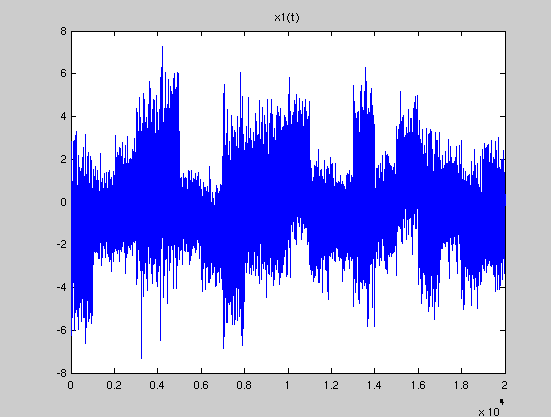
\includegraphics[width=5cm]{images/x1.png}}
	\subfloat[\label{l0pvs}]{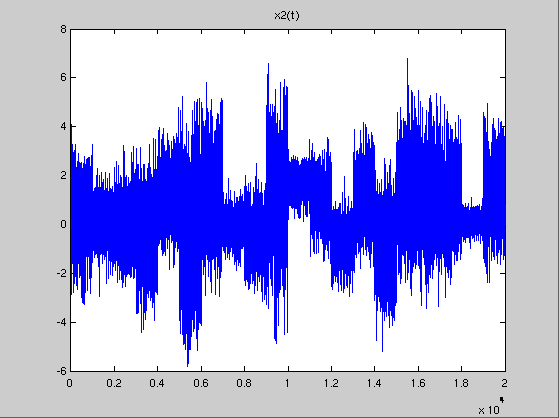
\includegraphics[width=5cm]{images/x2.png}}
	\subfloat[\label{l0pvs}]{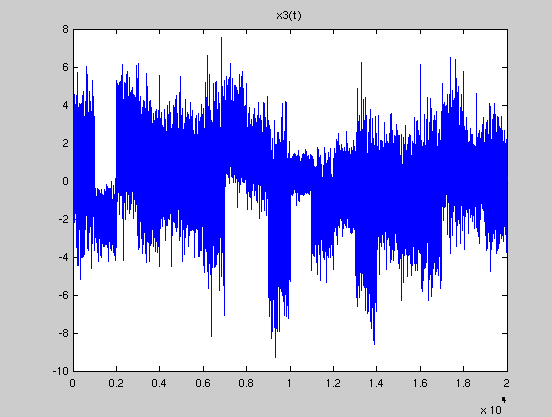
\includegraphics[width=5cm]{images/x3.png}} \\
	\subfloat[\label{l0pvs}]{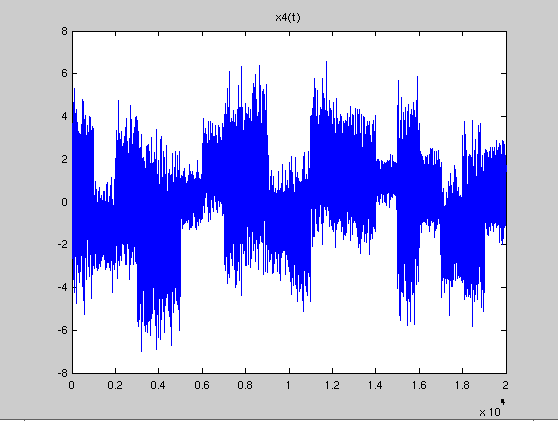
\includegraphics[width=5cm]{images/x4.png}} 
	\subfloat[\label{l0pvs}]{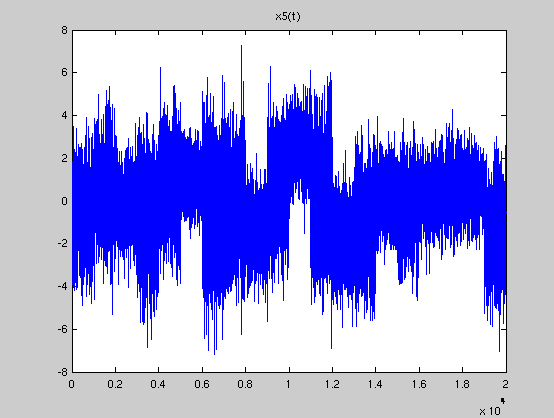
\includegraphics[width=5cm]{images/x5.png}} 
	\subfloat[\label{l0pvs}]{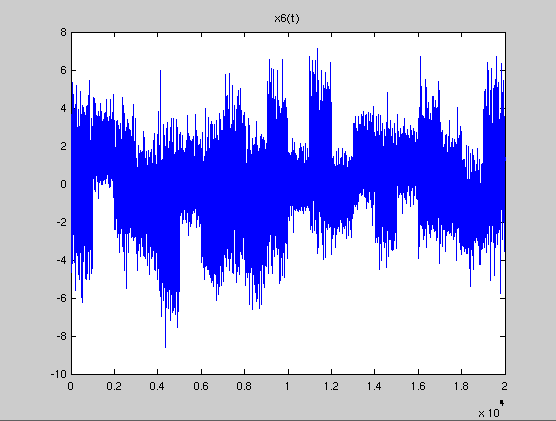
\includegraphics[width=5cm]{images/x6.png}} \\
	\subfloat[\label{l0pvs}]{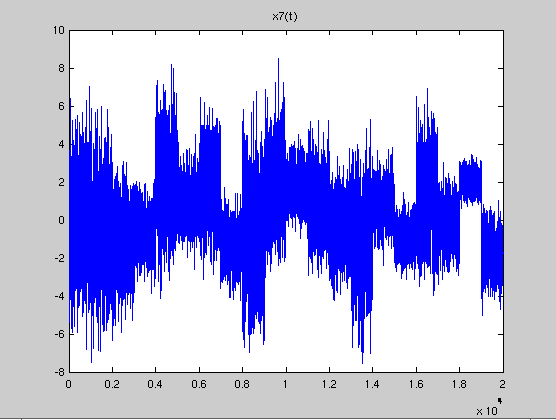
\includegraphics[width=5cm]{images/x7.png}} 
	\subfloat[\label{l0pvs}]{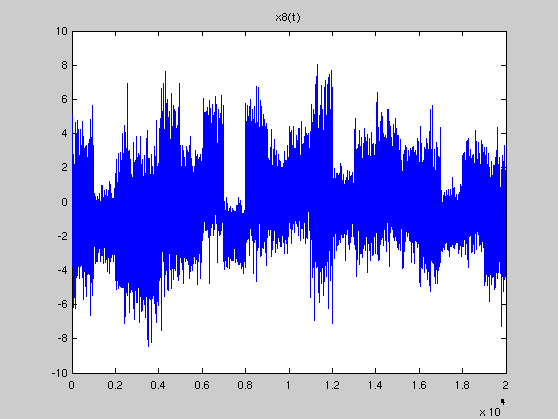
\includegraphics[width=5cm]{images/x8.png}}
	\subfloat[\label{l0pvs}]{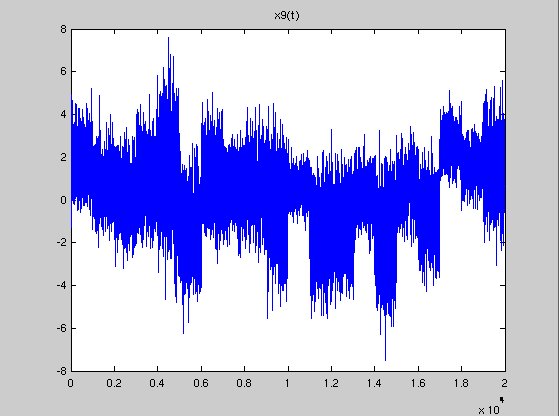
\includegraphics[width=5cm]{images/x9.png}} \\
	\subfloat[\label{l0pvs}]{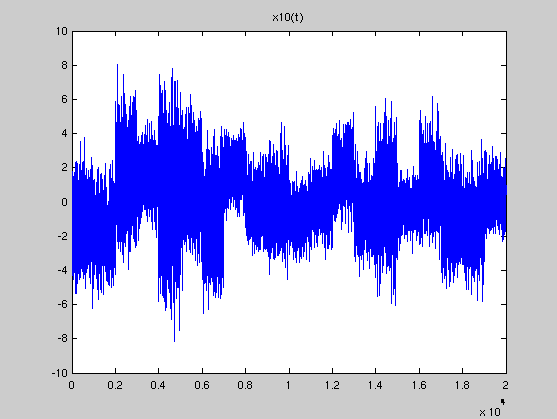
\includegraphics[width=5cm]{images/x10.png}}
	\caption{ Plots of each of the 10  (a)-(j) components with stationary and non-stationary included }
\end{figure}


\subsection{Experiments}

For the next experiments the number of expoches is set to 25. If one assume the number stationary sources in the dataset is $dd=3$, the plot of each component looks like:
\begin{figure}[H]
	\centering
	\subfloat[\label{test1}]{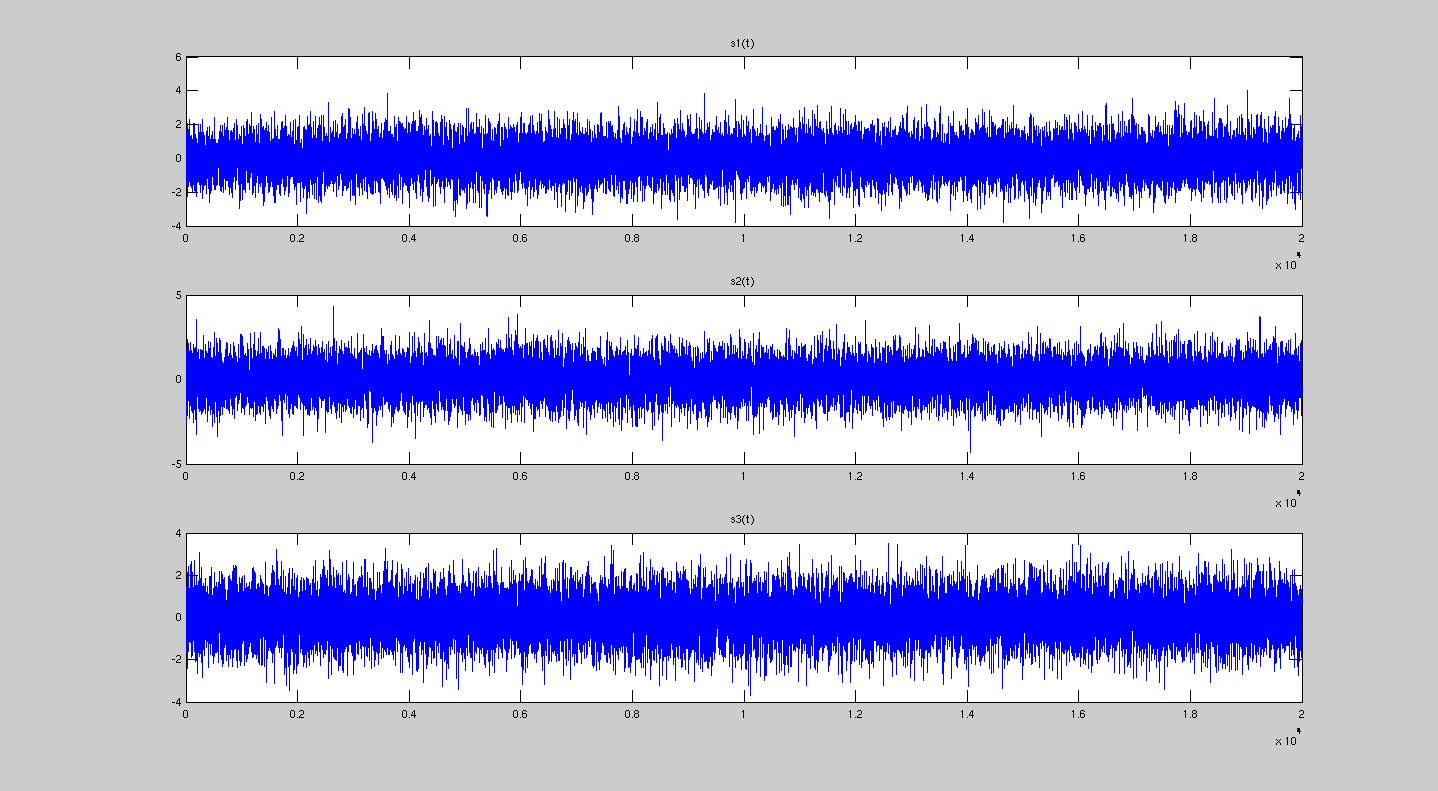
\includegraphics[width=\textwidth]{images/s1_3.png}}
	\caption{ Plot if number of stationary sources is set to 3.}
\end{figure}

\begin{figure}[H]
	\centering
	\subfloat[\label{test1}]{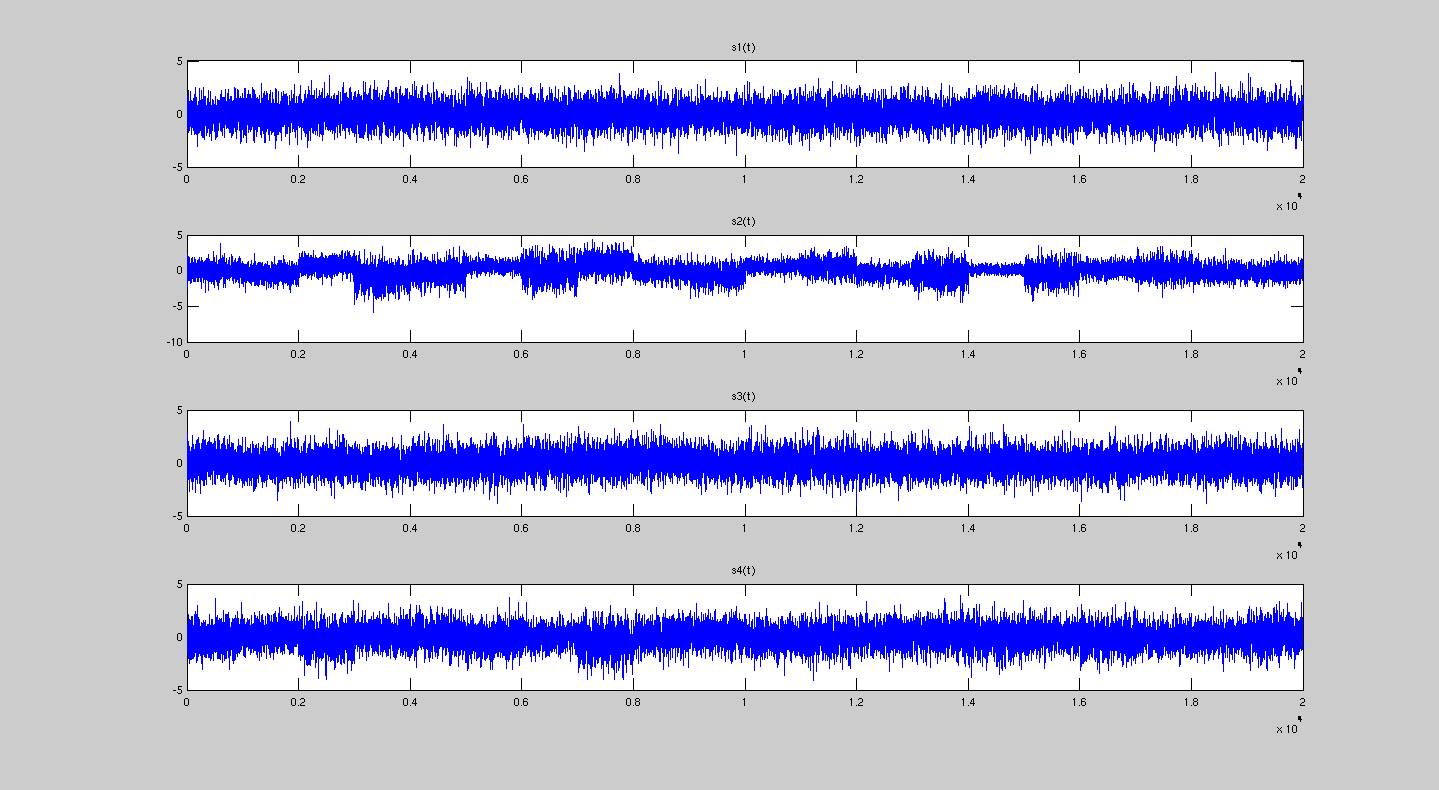
\includegraphics[width=\textwidth]{images/s1_4.png}}
	\caption{ Plot if number of stationary sources is set to 4.}
\end{figure}


In the next plot the number of stationary sources is incremnted to $dd=5$:

\begin{figure}[H]
	\centering
	\subfloat[\label{test1}]{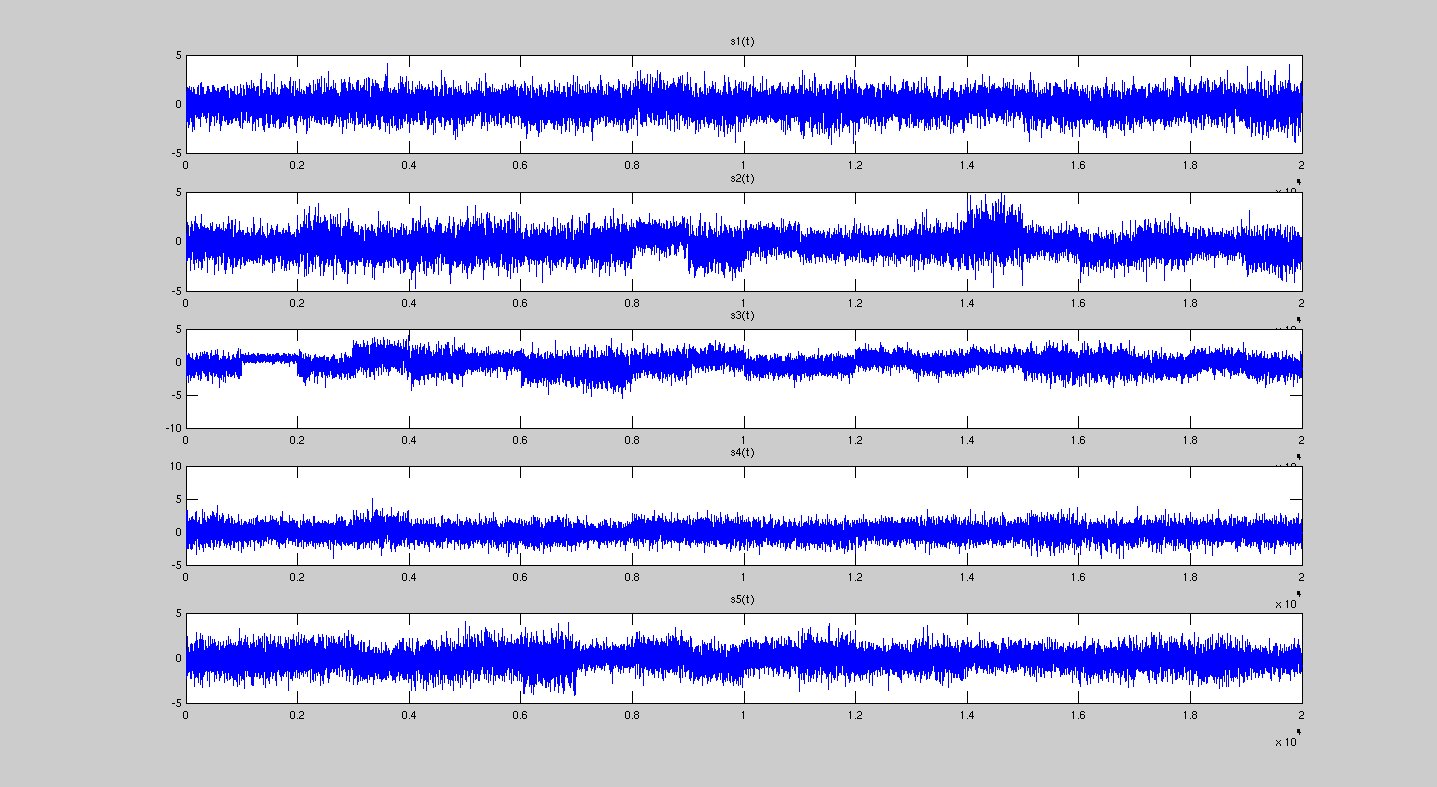
\includegraphics[width=\textwidth]{images/s1_5.png}}
	\caption{ Plot if number of stationary sources is set to 5.}
\end{figure}

\begin{figure}[H]
	\centering
	\subfloat[\label{test1}]{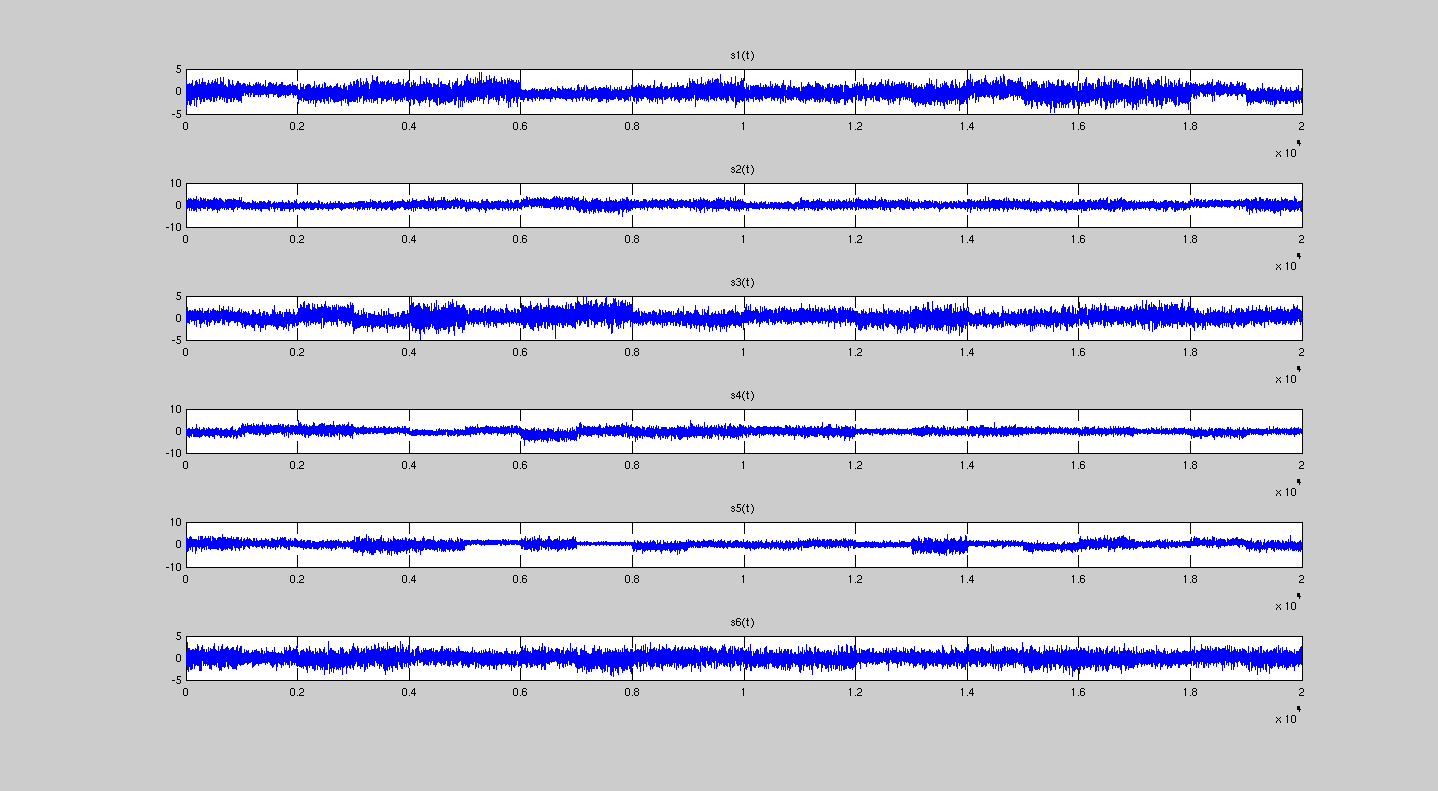
\includegraphics[width=\textwidth]{images/s1_6.png}}
	\caption{ Plot if number of stationary sources is set to 6.}
\end{figure}


In the next experiment, the number of stationary sources is incremnted to $dd=7$:


\begin{figure}[H]
	\centering
	\subfloat[\label{test1}]{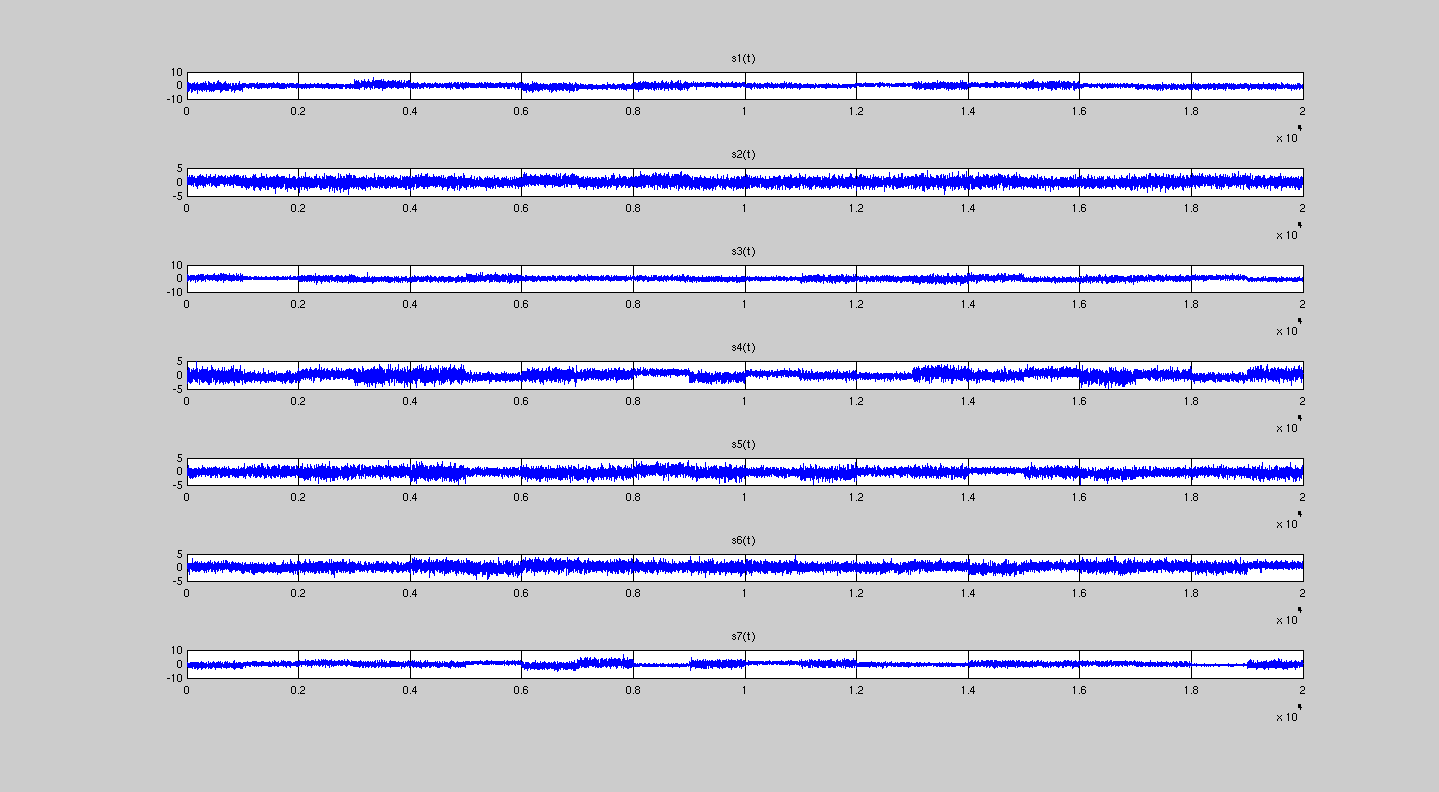
\includegraphics[width=\textwidth]{images/s1_7.png}}
	\caption{ Plot if number of stationary sources is set to 7.}
\end{figure}


\subsection{Number of stationary sources and projection}
If one compare the different plots from $dd=3$ to $dd=7$ the non-stationariy sources appear more and more.
Assuming the stationary sources coming from the same underlying distribution over the time-series, the best choice of the number of stationary sources ist 3.
\newline \newline

The projectionmatrix $B^s$ \newline

$
\begin{matrix}

    0.6581 &  -0.6022 &  -0.0495 &   0.6484 &  -0.1115 &   0.3517 &   0.6469 &  -0.3847 &   0.5758 &	0.0258 \\
   -0.0397 &   0.4733 &   0.2207 &  -0.1916 &  -0.1813 &  -0.3004 &  -0.1542 &  -0.2849 &  -0.6388 &	-0.4793 \\
    0.2932 &  -0.2916 &  -0.4973 &   0.7134 &   0.5037 &  -0.3822 &  0.0260 &  -0.3462  &  0.5083  &    0.1465

\end{matrix}
$



\newpage
\section{Uniqueness and identifiability of the SSA model}

\subsection*{$\left(a^\star\right)$}

\paragraph{The mixing matrix $A$ can in general not be identified exactly.}

The problem of identifying the mixing matrix $A$ uniquely is that any linear combination of a stationary time series is again stationary.
Furthermore, any linear combination of a stationary and non-stationary time series is non-stationary as-well.
Thus, even if we find an unmixing matrix $\hat B$ which separates the signal into its stationary and non-stationary part, one cannot be sure to have found the true unmixing matrix, because the basis of the stationary and non-stationary spaces can only be identified up to an arbitrary linear transformation within these spaces.
Having said that, a short example follows:

Assume a 3-dimensional source with 2 stationary sources and as mixing matrix the identity $A=I$:
\begin{eqnarray}
	\left(
		\begin{array}{c}
		x_1(t)\\
		x_2(t)\\
		x_3(t)		
		\end{array}
	\right) &=& A \left(
		\begin{array}{c}
			s^s_1(t)\\
			s^s_2(t)\\
			s^n_1(t)
		\end{array}
	\right)
\end{eqnarray}

Obviously, the identity matrix would also be a perfect unmixing matrix $\hat B = I$.
However, we cannot distinguish that solution from another solution where the 2 stationary sources are permuted:
\begin{eqnarray}
	\left(
		\begin{array}{c}
		x_1(t)\\
		x_2(t)\\
		x_3(t)		
		\end{array}
	\right) &=& A \cdot \left(
		\begin{array}{ccc}
		0&1&0\\
		1&0&0\\
		0&0&1
		\end{array}
	\right) \cdot \left(
		\begin{array}{c}
			s^s_1(t)\\
			s^s_2(t)\\
			s^n_1(t)
		\end{array}
	\right)
\end{eqnarray}
$\hat B=I$ would again separate the stationary and non-stationary space perfectly but not get the order right.
Consequently, matrix $A$ cannot be identified exactly.

\paragraph{Restriction on solutions of unmixing matrix.}
Assuming that we have found an unmixing matrix $\hat B = \hat A^{-1}$, then we also get an approximation of the stationary and non-stationary space $\hat A^s$ and $\hat A^n$. Since $\hat A$ has full rank we can express the true mixing matrix $A$ the following way:
\begin{eqnarray}
	A^s &=& \hat A^s M_1 + \hat A^n M_2\\
	A^n &=& \hat A^s M_3 + \hat A^n M_4\\
	\left(
		\begin{array}{c}
			\hat s^s\\
			\hat s^n 
		\end{array}
	\right) &=& \hat B A \left (
		\begin{array}{c}
			s^s\\
			s^n 
		\end{array}
	\right )\\
	&=& \left(
		\begin{array}{cc}
			M_1& M_3\\
			M_2 & M_4 \\
		\end{array}
	\right) \cdot \left(
		\begin{array}{c}
			s^s\\
			s^n
		\end{array}
	\right)
\end{eqnarray}

Since $\hat s^s$ shall be stationary, we mustn't mix in some non-stationary parts.
Thus, $M_3=0$.
The other matrices can be arbitrarily chosen.
That implies:
\begin{eqnarray}
	A^s &=& \hat A^s M_1 + \hat A_n M_2\\
	A^n &=& \hat A^n M_4
\end{eqnarray}

Consequently, the stationary space cannot be retrieved but it is possible to retrieve the non-stationary space up to an linear transformation of its basis.

\subsection*{$\left( b^\star \right)$}

To show: Given the column span of $A^n$ the mixing model is uniquely determined.

\begin{proof}
	The idea behind the proof is that we can only solve the unmixing problem up to an multiplicative factor $\left(
		\begin{array}{cc}
			M_1& 0\\
			M_2 & M_4 \\
		\end{array}
	\right)$.
	By solving the mixing problem with the column span $A^n$ and some additionally chosen vectors instead of $A^s$, we also obtain a solution for the original mixing problem $A=\left[ A^s \mid A^n \right]$.
	Given the column span $A^n$ we can extend it to a basis of dimension $D$.
	Let $\tilde A^s$ denote the newly added basis vectors.
	$\tilde A = \left [ \tilde A^s \mid A^n \right]$ is then used as mixing matrix:
	\begin{eqnarray}
		x(t) &=& \tilde A \left(
		\begin{array}{c}
			s^s(t)\\
			s^n(t)
		\end{array}
		\right)
	\end{eqnarray}
	For this problem we find, we find a unmixing matrix $\hat B$ such that:
	\begin{eqnarray}
		\hat B x(t) = \left(
		\begin{array}{cc}
			M_1& 0\\
			M_2 & M_4 \\
		\end{array}
	\right) \cdot  \left(
		\begin{array}{c}
			s^s(t)\\
			s^n(t)
		\end{array}
		\right)
	\end{eqnarray}
	
	By showing that $\hat B$ is also a solution for the original problem, we prove the equivalancy of the two problems and thus show that the mixing model is uniquely determined by its column span.
	
	Since the columns of $\tilde A$ are a basis we can find a solution to the following problem:
	\begin{eqnarray}
		A^s &=& \tilde A^s Q_1 + A^n Q_2	
	\end{eqnarray}
	
	And now
	\begin{eqnarray}
		\hat B A &=& \left(
		\begin{array}{cc}
			M_1& 0\\
			M_2 & M_4 \\
		\end{array}
		\right) \left[
		\begin{matrix}
		(\tilde A^s)^{-1}\\
		\hline
		(A^n)^{-1}		
		\end{matrix} \right] \cdot \left  [ \tilde A^s Q_1 + A^n Q_2 \mid A^n \right] \\
		&=&  \left(
		\begin{array}{cc}
			M_1& 0\\
			M_2 & M_4 \\
		\end{array}
		\right) \cdot \left(
		\begin{array}{cc}
			Q_1& 0\\
			Q_2 & I \\
		\end{array}
		\right)\\
		&=& \left(
		\begin{array}{cc}
			M_1 \cdot Q_1& 0\\
			M_2\cdot Q_1 + M_4 \cdot Q_2 & M_4 \\
		\end{array}
		\right)\\
		&=&  \left(
		\begin{array}{cc}
			\tilde M_1 & 0\\
			\tilde M_2 & M_4 \\
		\end{array}
		\right)
	\end{eqnarray}
	Consequently, $\hat B$ is also a solution for the mixing matrix $A$ and thus the problem is completely determined by the cloumn span of $A^n$.
\end{proof}

\end{document}
